\section{Introduction}
\begin{frame}
  \frametitle{Introduction}
\end{frame}

\begin{frame}
  \frametitle{Scenario}
  \begin{itemize}
    \item mmWave
      \begin{itemize}
        \item Multicell\footnote{mitigate path loss and shadowing}
      \end{itemize}
    \item Downlink eMBB and URLLC
      \begin{itemize}
        \item Puncturing\footnote{improve spectrum efficiency for sparse URLLC traffic}
        \item Hybrid\footnote{accommodate demands for bursty URLLC traffic}
      \end{itemize}
  \end{itemize}
\end{frame}

\begin{frame}
  \frametitle{Sparse URLLC Traffic}
  \begin{itemize}
    \item As the adoption of autonomous vehicles\footnote{include private cars and public transits} and drone delivery is still minor, URLLC downlink control traffic is rather dispersed.
    \item In this regard, having a dedicated channel in URLLC service wastes spectral resources, and such waste \highlight{scales linearly} with the number of base stations in the network.
  \end{itemize}
\end{frame}

\begin{frame}
  \begin{itemize}
    \item Do note that the discussion is applicable to any wireless systems serving two heterogeneous qualities of service (QoS) using short-wavelength technology.
  \end{itemize}
\end{frame}

\begin{frame}
  \frametitle{Contributions}
  \begin{itemize}
    \item A novel \highlight{linear} model for URLLC puncturing eMBB traffic in multicell networks is introduced, upon which optimality analysis for the multiplexing procedure is conducted.
    \item The proportional fairness algorithm's asymptotical optimality \cite{KW02} is generalized for eMBB resource allocation in multiconnectivity-based networks.
    \item The URLLC problem's optimal substructure is proved.
    \item A $\frac{\maxCostOneCur}{\minCostOneCur}$-approximation algorithm, the nearest association algorithm, that jointly schedules URLLC resources and links in multicell networks is proposed.
    \item An optimal algorithm, the opportunistic nearest association algorithm, which allocates URLLC resources in single-cell networks is derived.
  \end{itemize}
\end{frame}

\begin{frame}
  \frametitle{Related Work}
  \begin{itemize}
    \item Current models for URLLC puncturing scheme in the literature are mostly non-linear \cite{BMATAMHH21}.
    \item Whilst proposed linear models are either intractable \cite{YZR21} or inappropriate \cite{AVS20} for discrete subchannel allocation with multiple URLLC users.
    \item Many \cite{BMATAMHH21, YZR21} heuristically optimize the URLLC problem at each time minislot, without analyzing the optimal substructure.
  \end{itemize}
\end{frame}

\begin{frame}
  \frametitle{System}
  \begin{itemize}
    \item Homogeneous base stations, mmWave, downlink transmission, OFDMA, multiple-input eMBB and single-input URLLC users.
    \item Saturated eMBB traffic \cite{S05}: Each eMBB user has \highlight{infinite} amount of data to be served.
    \item Strict URLLC constraint: Each URLLC has an amount of data required to be served within a minislot.
    \item The system aims to maximize eMBB total average rate and fairness while satisfying URLLC demands.
  \end{itemize}
\end{frame}

\begin{frame}
  \frametitle{Multicell}
  \begin{figure}
    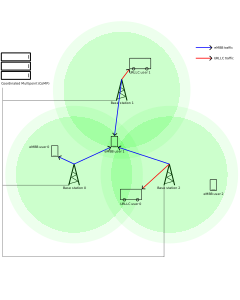
\includegraphics[width=0.5\textwidth]{model_multicell}
    \caption{Multicell model}
  \end{figure}
\end{frame}

\begin{frame}
  \begin{figure}
    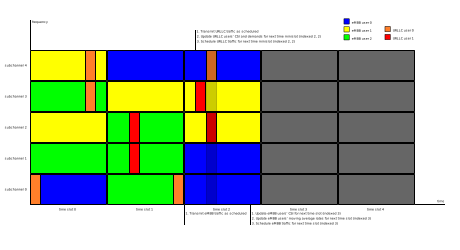
\includegraphics[width=1.05\textwidth]{framework_singlecell}
    \caption{Singlecell framework}
  \end{figure}
\end{frame}
